%%%%%%%%%%%%%%%%%%%%%%%%%%%%%%%%%%%%%%%%%
% Dreuw & Deselaer's Poster
% LaTeX Template
% Version 1.0 (11/04/13)
%
% Created by:
% Philippe Dreuw and Thomas Deselaers
% http://www-i6.informatik.rwth-aachen.de/~dreuw/latexbeamerposter.php
%
% This template has been downloaded from:
% http://www.LaTeXTemplates.com
%
% License:
% CC BY-NC-SA 3.0 (http://creativecommons.org/licenses/by-nc-sa/3.0/)
%
%%%%%%%%%%%%%%%%%%%%%%%%%%%%%%%%%%%%%%%%%

%----------------------------------------------------------------------------------------
%	PACKAGES AND OTHER DOCUMENT CONFIGURATIONS
%----------------------------------------------------------------------------------------

\documentclass[final,hyperref]{beamer}

\usepackage[orientation=portrait,size=a0,scale=0.8]{beamerposter} % Use the beamerposter package for laying out the poster with a portrait orientation and an a0 paper size

\usetheme{I6pd2} % Use the I6pd2 theme supplied with this template

\usepackage[english]{babel} % English language/hyphenation

\usepackage{amsmath,amsthm,amssymb,latexsym} % For including math equations, theorems, symbols, etc
\usepackage{algorithm2e}
\usepackage{tikz}
%\usepackage{times}\usefonttheme{professionalfonts}  % Uncomment to use Times as the main font
%\usefonttheme[onlymath]{serif} % Uncomment to use a Serif font within math environments

\boldmath % Use bold for everything within the math environment
\usepackage{xcolor}
\usepackage{booktabs} % Top and bottom rules for tables

\graphicspath{{figures/}} % Location of the graphics files

\usecaptiontemplate{\small\structure{\insertcaptionname~\insertcaptionnumber: }\insertcaption} % A fix for figure numbering

\newcommand{\argmin}[1]{\underset{#1}{\operatorname{argmin}}\;}
\newcommand{\argmax}[1]{\underset{#1}{\operatorname{argmax}\,\operatorname{min}}\;}
\def\mb{\mathbb}
\def\mf{\mathbf}

%----------------------------------------------------------------------------------------
%	TITLE SECTION 
%----------------------------------------------------------------------------------------

\title{\huge Artificial Bee Colony In Optimization} % Poster title

\author{Alexandr Ivanov} % Author(s)

\institute{MIPT DCAM} % Institution(s)

%----------------------------------------------------------------------------------------
%	FOOTER TEXT
%----------------------------------------------------------------------------------------

\newcommand{\leftfoot}{https://github.com/Avi2011class/Artificial-bee-colony} % Left footer text

\newcommand{\rightfoot}{avi2011class@yandex.ru} % Right footer text

%----------------------------------------------------------------------------------------

\begin{document}

\addtobeamertemplate{block end}{}{\vspace*{2ex}} % White space under blocks

\begin{frame}[t] % The whole poster is enclosed in one beamer frame

\begin{columns}[t] % The whole poster consists of two major columns, each of which can be subdivided further with another \begin{columns} block - the [t] argument aligns each column's content to the top

\begin{column}{.02\textwidth}\end{column} % Empty spacer column

\begin{column}{.465\textwidth} % The first column

%----------------------------------------------------------------------------------------
%	ABSTRACT and INTRODUCTION
%----------------------------------------------------------------------------------------

\begin{block}{Abstract}

\begin{itemize}
	\item 
		Abstract Swarm intelligence is a research branch that models the population of
		interacting agents or swarms that are able to self-organize. An ant colony, a flock of
		birds or an immune system is a typical example of a swarm system. Bees’ swarming
		around their hive is another example of swarm intelligence. Artificial Bee Colony
		(ABC) Algorithm is an optimization algorithm based on the intelligent behaviour of
		honey bee swarm. In this work, ABC algorithm is used for optimizing different 
		multivariable functions.
\end{itemize}

\end{block}

%----------------------------------------------------------------------------------------
%       INTRODUCTION
%----------------------------------------------------------------------------------------

\begin{block}{Introduction}
	\quad Several modern heuristic algorithms have been developed for solving combinatorial
	and numeric optimization problems. While an algorithm working with a set
	of solutions and trying to improve them is called population based, the one using
	multiple iterations to approach the solution sought is named as iterative algorithm.
	If an algorithm employs a probabilistic rule for improving a solution then it is called
	probabilistic or stochastic. Another classification can be made depending on the nature 
	of phenomenon simulated by the algorithm. This type of classification mainly has two
	important groups of population based algorithms: evolutionary algorithms (EA) and
	swarm intelligence based algorithms. The most popular EA is Genetic Algorithm
	(GA). GA attempts to simulate the phenomenon of natural evolution. In natural
	evolution, each species searches for beneficial adaptations in an everchanging 
	environment. 

	\quad Several approaches have been proposed to model the specific intelligent 
	behaviours of honey bee swarms and applied for solving combinatorial type problems.
	Bee colony may be considered as a dynamical system of robots gathering
	information from an environment and adjusting its behaviour in accordance to it. 	
	Usually, all these robots
	are physically and functionally identical. The swarm possesses a significant tolerance; 
	the failure in a single agent does not stop the performance of the whole system. 
	The individual robots, like insects, have limited capabilities and limited knowledge 
	of the environment. On the other hand, the swarm develops collective intelligence. 

	\quad Here one approach to optimization in convex sets will be considered.
	In this case, completely identical robots are located inside a certain set K, 
	and the movements are calculated as follows

	$$ P_{t+1} = P_t + c_1 \cdot (L - P_t) \cdot l_t + c_2 \cdot (G - P_t) \cdot g_t $$
	

\end{block}

%----------------------------------------------------------------------------------------
%	FORMAL PROBLEM
%----------------------------------------------------------------------------------------
            
\begin{block}{Problem formulation}

\begin{itemize}
	\item 
		$ \mb{Q} \subseteq \mb{R}^n $ is convex
	\item
		$ f: \mb{Q} \to \mb{R}, \ \mb{Q} \subset \mb{R}^n $
	\item
		$f$ is continuous on the set $\mb{Q}$ with the exception of the finite union of connected zero measured sets
	\item
		$ x^* = \argmin{x \in Q} f(x)$

\end{itemize}

\end{block}

%----------------------------------------------------------------------------------------
%	MATHEMATICAL SECTION
%----------------------------------------------------------------------------------------

\begin{block}{Given to blackbox}


\begin{itemize}
	\item 
		$f$ - function to optimize
		$N$ - the number of optiomazation steps
		$K$ - the number of swarms
	\item
		$l(t),\ g(t)$ - dependencies of attraction coefficients to local 
		and global minimum on time 
	\item
		$\sigma(t)$ - dependence of random factor on time 
\end{itemize}

Recommended functions is: 
$$ l(t) = \alpha_1 \cdot e^{-\gamma t},       \; \; 0.1 \leq \alpha_1 \leq 0.4 $$
$$ g(t) = 2 \alpha \cdot (1 - e^{-\gamma t}),   \; \; 0.05 \leq \alpha_2 \leq 0.3 $$
$$ \sigma(t) = \beta \cdot \mathbf{diam}(\mb{Q}) \cdot e^{-\gamma t},  \; \;  0 \leq \beta \leq 0.1   $$
$$ \gamma \sim N $$

\end{block}

%----------------------------------------------------------------------------------------
%	BLACKBOX
%----------------------------------------------------------------------------------------



\begin{block}{Blackbox algorithm}
You can see python3 code on \href{https://github.com/Avi2011class/Artificial-bee-colony/blob/master/modules/ABC.py}{github}.

\begin{algorithm}[H]

	
	\SetKwData{Left}{left}\SetKwData{This}{this}\SetKwData{Up}{up}
	\SetKwFunction{Union}{Union}\SetKwFunction{FindCompress}{FindCompress}
	\SetKwInOut{Input}{input}\SetKwInOut{Output}{output}
	
	\BlankLine
	\KwIn{$f$ - function to minimize, $\mb{Q}$ - optimization area, $N$ - number of steps, 
			$K$ - number of swarms, $l(t)$, $g(t)$, $\sigma(t)$ - optimize functions like a recommended}
	\KwOut{$x^* \simeq \argmin{x \in Q} f(x)$}

	\BlankLine

	\For{i=1\ldots $K$} {
		$ bee_i \leftarrow$ random point from $\mb{Q}$ \\
		$ lres_i \leftarrow Bee_i $
		$ lvalue \leftarrow f(lres_i) $
	}
	res $\leftarrow$ random point from Q

	\BlankLine

	\For{iter = 1 \ldots $N$} {

		\For{j=1 \ldots $K$} {
			$c_1, c_2 \leftarrow Random([0 \ldots 1])$ \\
			\BlankLine
			$V_j \leftarrow (lres_i - bee_i) \cdot l(iter) \cdot c_1 + (res - bee_i) \cdot g(iter) \cdot c_2 
						+ N(0, \sigma(iter)) $ 
		}
		
		\BlankLine 
		\For{j=1 \ldots $K$}{
			\If{$bee_i + V_i \in \mb{Q}$} {
			$bee_i \leftarrow bee_i + V_i$
			\If {$f(bee_i) \leq f(lres_i)$ } {
				$lres_i \leftarrow bee_i$
			}
			}
		}

		\BlankLine
		
		\For{j=1 \ldots $K$} {
			$res \leftarrow min(res, lres_i)$
		}

	}
	
	\BlankLine
	
	\Return res

	\caption{ABC optimizer}
\end{algorithm}


\end{block}
%----------------------------------------------------------------------------------------
%	RESULTS
%----------------------------------------------------------------------------------------

\begin{block}{Results}

	
	Four functions were optimized by three global methods: Genetic Algorithm(GA), Artificial Bee Colony algorithm(ABC), Annealing Simulation(AS).

	The functions are:
	\begin{enumerate}
		\item
			Qadratic function
			$$ f_1(x, y) = \| (x, y) - (0, 0) \|_2 $$
		\item
			Function with a large number of minima and semi-regular structure
			$$ f_2(x, y) = 0.00005 \cdot (x^2 + y^2) + 10\sin(x/30) + 10\sin(y/30) $$
		\item
			(Schwefel’s construction) Very complex function with a single global minimum
			$$ f_3(x, y) = 837.9658 - x \cdot \sin(\sqrt(|x|)) - y \cdot \sin(\sqrt(|y|)) $$
		\item 
			$f_4$ is loss function for logistic regression with polynomial (quadratic) features for 
			two clases from popular iris dataset. 
	\end{enumerate}

	In 1-3 cases, the $\mb{Q} = \{ x,y \in \mb{R} \vert -500 \leq x, y \leq 500 \} $\\
	Here is the number of iterations for custom ABC algorithm ($K=5, \alpha_1=\alpha_2=0.2$), GA from DEAP python library and AS from scipy.optimize with default paramenters. Stop criteria is $\|x-x^*\| < 0.1$


	\begin{table}
 		\begin{tabular}{r|c c c c}
		\toprule
			\textbf{ Method } & $f_1$ & $f_1$ & $f_3$ & $f_4$ \\
		\midrule
			ABC  \;\; & \;\;  21  \;\; & \;\;  85   \;\; & \;\;   431   \;\; & \;\;  1888      \\
			GA   \;\; & \;\;  17  \;\; & \;\;  42   \;\; & \;\;   397   \;\; & \;\;  913       \\
			AS   \;\; & \;\;  50  \;\; & \;\;  118  \;\; & \;\;  1631   \;\; & \;\;  7210      \\
		\bottomrule

		\end{tabular}

		\caption{Median number of iterations for different optimizers}
	\end{table}
     	

	\begin{table}
 		\begin{tabular}{r|c c c c}
		\toprule
			\textbf{ Method } & $f_1$ & $f_1$ & $f_3$ & $f_4$ \\
		\midrule
			ABC  \;\; & \;\;  2.82  \;\; & \;\;  1.32   \;\; & \;\;   1.00   \;\; & \;\;   3.74      \\
			GA   \;\; & \;\;  3.48  \;\; & \;\;  3.01   \;\; & \;\;   6.29   \;\; & \;\;   1.00      \\
			AS   \;\; & \;\;  1.00  \;\; & \;\;  1.00   \;\; & \;\;   3.51   \;\; & \;\;   4.23      \\
		\bottomrule

		\end{tabular}

		\caption{Median machine time in relative units}
	\end{table}
 

\end{block}


%----------------------------------------------------------------------------------------

\end{column} % End of the first column

\begin{column}{.03\textwidth}\end{column} % Empty spacer column
 
\begin{column}{.465\textwidth} % The second column


%----------------------------------------------------------------------------------------
%	SAMPLE FUNCTIONS
%----------------------------------------------------------------------------------------

\begin{block}{Sample functions}
	
\begin{figure}[H]
	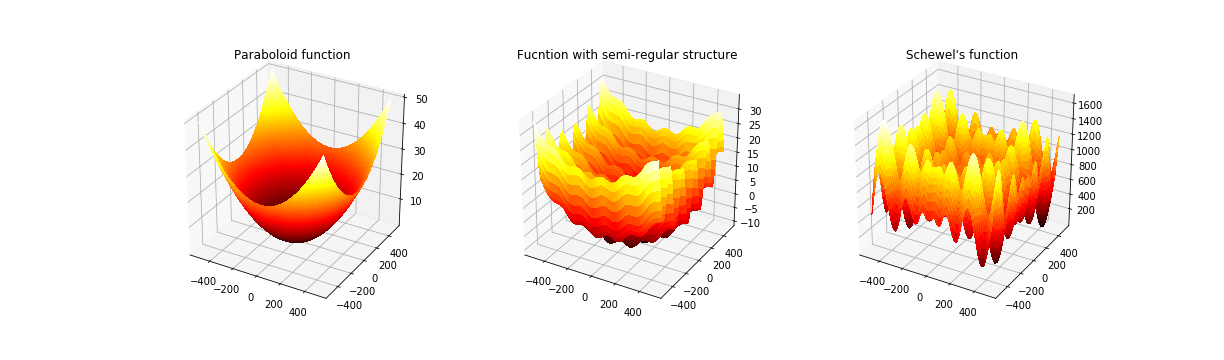
\includegraphics[width=1.0\linewidth]{samples.png}
	\caption{$f_1, f_2, f_3$ 3d-plots}
\end{figure}

\end{block}


%---------------------------------------------------------------------------------------
% 	FIGURES
%---------------------------------------------------------------------------------------

\begin{block}{Results: Figure}

\begin{figure}[H]
	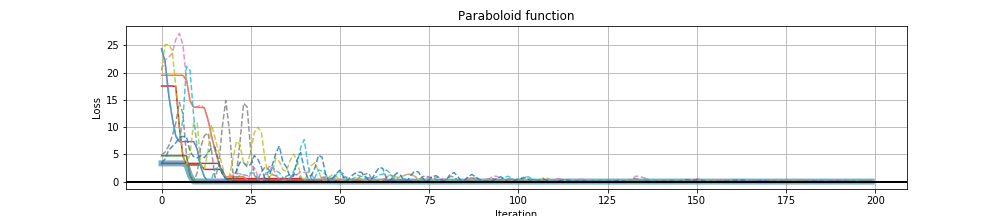
\includegraphics[width=0.9\linewidth]{paraboloid_tr.png}
	\caption{ABC behavior in paraboloid function}
\end{figure}

\begin{figure}[H]
	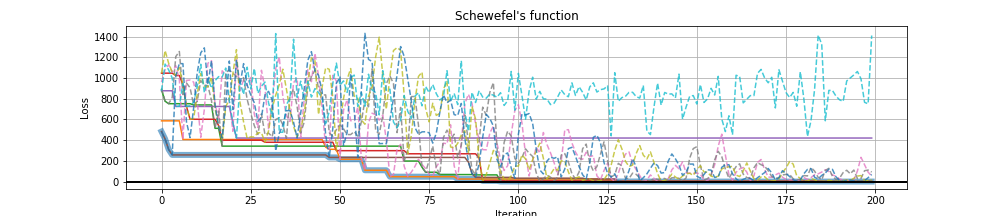
\includegraphics[width=0.9\linewidth]{schevefel_tr.png}
	\caption{ABC behavior in Schewefel's function}
\end{figure}


\end{block}

%----------------------------------------------------------------------------------------
%	APPLICATION
%----------------------------------------------------------------------------------------
\begin{block}{Application}
	An interesting application of the algorithm is the optimization of functions defined 
	on flows in some graphs. If in some network sources and sinks are fixed, together with 
	their capacities, then the space of all possible flows on it will turn out to be a 
	linear relative to the sum operator over all edges.
	Moreover, this remains true if certain parts of the flow are fixed, this structures are 
	called "Semidefinite flows". There is finite-dimensional system is the space.
	\begin{figure}[H]
	\begin{center}
		\begin{tikzpicture}[scale=0.3]
			\tikzstyle{every node}+=[inner sep=0pt]
			\draw [black] (18,-23.5) circle (3);
			\draw (18,-23.5) node {$3$};
			\draw [black] (33.8,-23.5) circle (3);
			\draw (33.8,-23.5) node {$4$};
			\draw [black] (30.9,-34.9) circle (3);
			\draw (30.9,-34.9) node {$12$};
			\draw [black] (32.9,-14.6) circle (3);
			\draw (32.9,-14.6) node {$5$};
			\draw [black] (42.7,-6.2) circle (3);
			\draw (42.7,-6.2) node {$15$};
			\draw [black] (57.8,-5.2) circle (3);
			\draw (57.8,-5.2) node {$13$};
			\draw [black] (52.3,-17.3) circle (3);
			\draw (52.3,-17.3) node {$7$};
			\draw [black] (42.7,-28.5) circle (3);
			\draw (42.7,-28.5) node {$6$};
			\draw [black] (6.8,-31.9) circle (3);
			\draw (6.8,-31.9) node {$14$};
			\draw [black] (6.8,-31.9) circle (2.4);
			\draw [black] (21.8,-5.2) circle (3);
			\draw (21.8,-5.2) node {$2$};
			\draw [black] (69,-13.6) circle (3);
			\draw (69,-13.6) node {$10$};
			\draw [black] (55.8,-34.9) circle (3);
			\draw (55.8,-34.9) node {$8$};
			\draw [black] (6.8,-9.5) circle (3);
			\draw (6.8,-9.5) node {$1$};
			\draw [black] (6.8,-9.5) circle (2.4);
			\draw [black] (73.6,-26.4) circle (3);
			\draw (73.6,-26.4) node {$9$};
			\draw [black] (73.6,-4.1) circle (3);
			\draw (73.6,-4.1) node {$11$};
			\draw [black] (69,-35.7) circle (3);
			\draw (69,-35.7) node {$16$};
			\draw [black] (21,-23.5) -- (30.8,-23.5);
			\fill [black] (30.8,-23.5) -- (30,-23) -- (30,-24);
			\draw [black] (33.06,-26.41) -- (31.64,-31.99);
			\fill [black] (31.64,-31.99) -- (32.32,-31.34) -- (31.35,-31.09);
			\draw [black] (24.8,-5.34) -- (39.7,-6.06);
			\fill [black] (39.7,-6.06) -- (38.93,-5.52) -- (38.88,-6.52);
			\draw [black] (40.42,-8.15) -- (35.18,-12.65);
			\fill [black] (35.18,-12.65) -- (36.11,-12.51) -- (35.46,-11.75);
			\draw [black] (8.67,-11.84) -- (16.13,-21.16);
			\fill [black] (16.13,-21.16) -- (16.02,-20.22) -- (15.24,-20.85);
			\draw (11.84,-17.92) node [left] {$11$};
			\draw [black] (9.68,-8.67) -- (18.92,-6.03);
			\fill [black] (18.92,-6.03) -- (18.01,-5.77) -- (18.28,-6.73);
			\draw (15.76,-7.95) node [below] {$15$};
			\draw [black] (45.69,-6) -- (54.81,-5.4);
			\fill [black] (54.81,-5.4) -- (53.98,-4.95) -- (54.04,-5.95);
			\draw [black] (66.012,-13.34) arc (-96.28434:-115.14556:65.385);
			\fill [black] (45.39,-7.54) -- (45.9,-8.33) -- (46.32,-7.42);
			\draw [black] (67.68,-16.294) arc (-26.86744:-36.70707:111.287);
			\fill [black] (57.63,-32.52) -- (58.5,-32.18) -- (57.7,-31.58);
			\draw [black] (71.49,-11.947) arc (151.30535:-136.69465:2.25);
			\draw (76.37,-12.6) node [right] {$0$};
			\fill [black] (71.83,-14.57) -- (72.29,-15.39) -- (72.77,-14.52);
			\draw [black] (66.07,-14.25) -- (55.23,-16.65);
			\fill [black] (55.23,-16.65) -- (56.12,-16.97) -- (55.9,-15.99);
			\draw [black] (27.92,-34.53) -- (9.78,-32.27);
			\fill [black] (9.78,-32.27) -- (10.51,-32.87) -- (10.63,-31.87);
			\draw (19.35,-32.74) node [above] {$19$};
			\draw [black] (15.6,-25.3) -- (9.2,-30.1);
			\fill [black] (9.2,-30.1) -- (10.14,-30.02) -- (9.54,-29.22);
			\draw (11.25,-27.2) node [above] {$3$};
			\draw [black] (35.578,-15.941) arc (57.76594:12.60449:15.272);
			\fill [black] (42.34,-25.53) -- (42.65,-24.64) -- (41.67,-24.86);
			\draw (40.51,-18.69) node [right] {$17$};
			\draw [black] (53.1,-33.58) -- (45.4,-29.82);
			\fill [black] (45.4,-29.82) -- (45.89,-30.62) -- (46.33,-29.72);
			\draw [black] (40.06,-29.93) -- (33.54,-33.47);
			\fill [black] (33.54,-33.47) -- (34.48,-33.53) -- (34,-32.65);
			\draw [black] (19.952,-21.225) arc (135.62332:106.07772:22.885);
			\fill [black] (19.95,-21.22) -- (20.87,-21) -- (20.15,-20.3);
			\draw [black] (49.33,-16.89) -- (35.87,-15.01);
			\fill [black] (35.87,-15.01) -- (36.59,-15.62) -- (36.73,-14.63);
			\draw [black] (53.85,-32.627) arc (-144.84807:-192.6573:15.701);
			\fill [black] (53.85,-32.63) -- (53.8,-31.68) -- (52.98,-32.26);
			\draw [black] (54.664,-19.134) arc (45.07422:-22.57959:12.058);
			\fill [black] (54.66,-19.13) -- (54.88,-20.05) -- (55.58,-19.34);
			\draw (58.71,-25.01) node [right] {$5$};
			\draw [black] (50.35,-19.58) -- (44.65,-26.22);
			\fill [black] (44.65,-26.22) -- (45.55,-25.94) -- (44.79,-25.29);
			\draw [black] (28.65,-32.91) -- (20.25,-25.49);
			\fill [black] (20.25,-25.49) -- (20.52,-26.39) -- (21.18,-25.64);
			\draw [black] (53.037,-36.067) arc (-68.75104:-118.25603:52.207);
			\fill [black] (9.4,-33.4) -- (9.87,-34.21) -- (10.34,-33.33);
			\draw (30.84,-40.08) node [below] {$4$};
			\draw [black] (18.61,-20.56) -- (21.19,-8.14);
			\fill [black] (21.19,-8.14) -- (20.54,-8.82) -- (21.52,-9.02);
			\draw [black] (33.9,-34.9) -- (52.8,-34.9);
			\fill [black] (52.8,-34.9) -- (52,-34.4) -- (52,-35.4);
			\draw [black] (71.342,-6.062) arc (-56.64048:-115.39448:11.274);
			\fill [black] (71.34,-6.06) -- (70.4,-6.08) -- (70.95,-6.92);
			\draw (66.04,-8.46) node [below] {$1$};
			\draw [black] (72.29,-6.8) -- (70.31,-10.9);
			\fill [black] (70.31,-10.9) -- (71.11,-10.4) -- (70.21,-9.96);
			\draw [black] (70.01,-16.42) -- (72.59,-23.58);
			\fill [black] (72.59,-23.58) -- (72.79,-22.65) -- (71.84,-22.99);
			\draw (72.06,-19.22) node [right] {$3$};
			\draw [black] (72.27,-29.09) -- (70.33,-33.01);
			\fill [black] (70.33,-33.01) -- (71.13,-32.52) -- (70.24,-32.07);
			\draw (70.6,-29.95) node [left] {$3$};
			\draw [black] (66.01,-35.52) -- (58.79,-35.08);
			\fill [black] (58.79,-35.08) -- (59.56,-35.63) -- (59.62,-34.63);
			\draw (62.49,-34.74) node [above] {$3$};
			\draw [black] (60.603,-4.136) arc (106.95741:81.00763:22.489);
			\fill [black] (60.6,-4.14) -- (61.51,-4.38) -- (61.22,-3.42);
		\end{tikzpicture}
		\end{center}
		\caption{Example of a semidefinite flow}
	\end{figure}

	The problem consists in constructing a correct flow that coincides on these edges with 
	a semidefinite flow on where some functional is minimal. \\

	Here we will use the following loss function
	$$ F = \sum\limits_{e \in \text{Edges}(\mf{G})} \text{Loss}_e(\text{Flow}(e)) $$
	$$ Loss_e(x) = -\arctan(-(x-\mu_e)) \cdot (x-\mu_e) + e^{-(x-\mu_e)} / \mu_e + e^{(x-2\mu_e)} / 2\mu_e  $$
	Where $\mu_e$ is the edge property.

	
	\begin{figure}[H]
		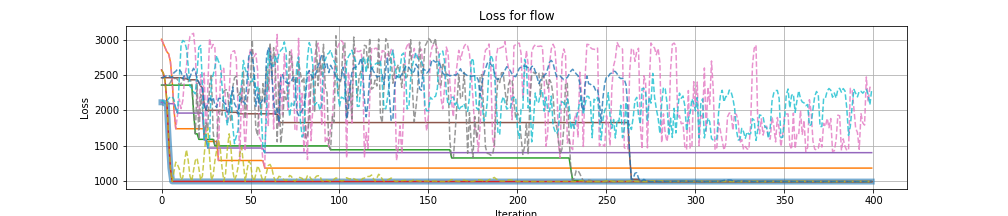
\includegraphics[width=1.0\linewidth]{flow_tr.png}
		\caption{The typical behavior of the algorithm on a given loss function}
	\end{figure}
	It works :-)

\end{block}

%----------------------------------------------------------------------------------------
%	CONCLUSION
%----------------------------------------------------------------------------------------

\begin{block}{Conclusion}

\begin{itemize}
	\item 
		\textcolor{green}{\textbf{+}} The algorithm does not have any requirements to the smoothness
						of the objective function
	\item	
		\textcolor{green}{\textbf{+}} It is possible to write a qualitative parallel implementation
	\item	
		\textcolor{green}{\textbf{+}} It is possible to leave the local minima using appropriate parameters
	\item
		\textcolor{green}{\textbf{+}} Good results can be obtained by using this method to search 
						for potential minima for further use of local optimization methods


	\item
		\textcolor{red}{\textbf{--}} The quality of work depends on the parameters that are difficult to select
	\item
		\textcolor{red}{\textbf{--}} If the parameters are incorrect, there is no chance of correct operation
	\item
		\textcolor{red}{\textbf{--}} A great waste of computer time on checking conditions if the budget set is not convex
	\item
		\textcolor{red}{\textbf{--}} In the case of convexity, the function is noticeably inferior to other methods

\end{itemize}

\end{block}

%----------------------------------------------------------------------------------------
%	MATERIALS
%----------------------------------------------------------------------------------------

\begin{block}{References}
\begin{enumerate}
	\item
		Pham, D.T., Karaboga, D.: Intelligent Optimisation Techniques. Springer, London (2000)
	\item
		Holland, J.H.: Adaptation in Natural and Artificial Systems. University of Michigan Press, Ann Arbor, MI (1975)
	\item
		Kennedy, J., Eberhart, R.C.: Particle swarm optimization. In: Proceedings of the 1995 IEEE
		International Conference on Neural Networks, vol. 4, pp. 1942–1948. IEEE Service Center,
		Piscat away (1995)
	\item
		Vodolazsky IA, Egorov AS, Krasnov AV Roaring intellect and its most common methods of 
		realization // Young scientist. - 2017. - № 4. - P. 147-153. - URL 
		https://moluch.ru/archive/138/38900/ (reference date: May 28, 2013).
	
\end{enumerate}

\end{block}


%----------------------------------------------------------------------------------------
%	CONTACT INFORMATION
%----------------------------------------------------------------------------------------

%\setbeamercolor{block title}{fg=black,bg=orange!70} % Change the block title color

\begin{block}{Contact Information}

\begin{itemize}
\item Web: \href{https://github.com/Avi2011class}{https://github.com/Avi2011class}
\item Email: \href{mailto:avi2011class@yandex.ru}{avi2011class@yandex.ru}
\end{itemize}

\end{block}

%----------------------------------------------------------------------------------------

\end{column} % End of the second column

\begin{column}{.015\textwidth}\end{column} % Empty spacer column

\end{columns} % End of all the columns in the poster

\end{frame} % End of the enclosing frame

\end{document}
